% DUET -- Design (DAC 2027 draft, 2026-10-21)
% Mechanisms = ~/nvmevirt_proposed/dm/ftl_proposed.c (NOTES_proposed.md), bit-identical to ftlsim mode=proposed
% with spill=2, spill_rp=1, spill_rp_clean=1. DRAM numbers: 92 GiB device, U=16, 1/8 budget.

\section{DUET Design}
\label{sec:design}

DUET maps every logical page through two levels (Figure~\ref{fig:design}).
A \emph{coarse map} keeps one entry per 64\,KiB IU, and a \emph{fine map}
keeps 4\,KiB fragments that override parts of an IU. The coarse map is always
in DRAM, so most reads need no mapping I/O (requirement (i)); fragments are
merged one IU at a time instead of one block at a time (ii); and small writes
go to fragments instead of RMW (iii).

\begin{figure}[t]
  \centering
  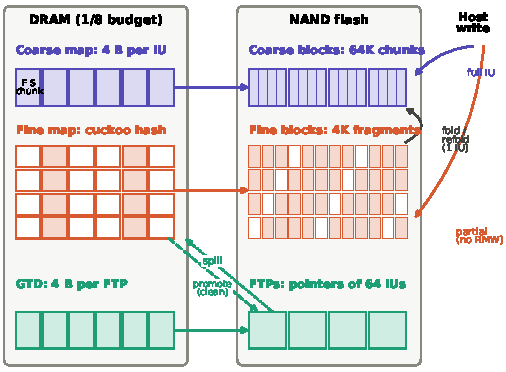
\includegraphics[width=\columnwidth]{figs/fig_design.pdf}
  \vspace{-6mm}
  \caption{DUET overview. The coarse map (one 4\,B entry per 64\,KiB IU, with
  has-fragments (F) and spilled (S) bits) points to 16-page chunks; the fine map,
  a cuckoo hash, points to 4\,KiB fragments. Fragment pointers of evicted IUs are
  spilled to flash translation pages (FTPs), located by the GTD, and promoted back
  clean on access. Fragments are merged one IU at a time (fold / refold).}
  \label{fig:design}
  \vspace{-4mm}
\end{figure}

\subsection{Two Mapping Granularities}
\textbf{Coarse map.} The logical space is divided into 64\,KiB IUs of 16
pages. Each IU is stored as a \emph{chunk} of 16 physically consecutive,
16-page-aligned pages in a \emph{coarse block}, so a 4\,B coarse entry holds
the chunk index plus two flag bits: \emph{has-fragments} and \emph{spilled}.
The coarse map takes 1/16 of a page-level table.

\textbf{Fine map.} A write smaller than an IU is written out of place as 4\,KiB
\emph{fragments} into separate \emph{fine blocks}. A fragment overrides the
corresponding page of its IU's chunk, which stays in place. The fine map is a
bucketized cuckoo hash table (two candidate buckets of four 8\,B
\{logical page, physical page\} entries), sized to whatever the DRAM budget
leaves after the coarse map. On our 92\,GiB device with a 1/8 budget, the coarse
map takes 5.6\,MiB and the table 5.5\,MiB, enough for fragments of about 3\% of
all logical pages.

\textbf{Read path.} A read first checks the coarse entry. If the
has-fragments bit is clear, the page is read from the chunk at offset
$\mathit{lpn} \bmod 16$. Otherwise one table lookup (at most two buckets)
returns the fragment if it exists, and the chunk page if not. A read thus needs
at most three DRAM accesses and one flash read; a mapping read occurs only for
spilled IUs (Section~\ref{sec:elastic}).

\textbf{Write path.} A write that covers a whole IU goes to the coarse
frontier as a new chunk; the old chunk and all fragments of the IU become
invalid. A partial write becomes fragments. A partial write that covers most of
an IU is completed right away (the missing pages are read and the whole IU is
written as a chunk) when this is cheaper than the fragments' expected cost.
That cost is estimated from the measured fraction of fragments that eventually
need a fold.

\subsection{Reclaiming Fragments without Block Merges}
Fragments leave the fine map in three ways, and none of them copies more than
one IU.

\textbf{Overwrite.} A later full-IU write invalidates the IU's fragments for
free. The same happens to a fragment when its page is rewritten, so hot small
writes keep cycling inside the fine blocks.

\textbf{Fold during fine GC.} When fine blocks run out, DUET picks a victim fine
block and, for each IU with live fragments in it, either copies the fragments
forward or \emph{folds} the IU: it reads the chunk and the $d$ fragments, writes
one new chunk, and frees all $d$ fragments. Folding costs one IU write ($U=16$
pages) and frees $d$ fine pages, whereas copying keeps the fragments and costs
the usual GC copy cost of the victim block. DUET folds when
$d \cdot v > U \cdot (P - v)$, where $v$ is the number of valid pages in the
victim and $P$ the pages per block, and prefers to keep recently written (hot)
fragments.

\textbf{Refold during coarse GC.} Coarse blocks are reclaimed by page-style
garbage collection with a cost-benefit victim policy. When GC relocates a chunk
whose IU has fragments, it writes the merged IU instead of the stale chunk, so
the fragments are freed at no extra program cost. On YCSB-A, 79\% of all
fragments leave the fine map this way.

Since every merge touches a single IU, its cost is bounded by 16 page copies
regardless of the erase-block size, unlike a hybrid FTL's block merge. DUET also
decides between fine and coarse GC by their cost, so the fine area grows when
fragments are rewritten often and shrinks to a few blocks under uniform random
writes.

\subsection{Elastic Fragment Mapping}
\label{sec:elastic}
The fine map has a fixed DRAM size, but the number of IUs with fragments does
not. A conventional design must fold IUs whenever the table fills, which turns
DRAM pressure into data copies. DUET instead lets the fine map \emph{spill} to
flash and come back.

\textbf{Spill.} The fragment pointers of IU $i$ have a fixed home in flash
translation page (FTP) $\lfloor i/64 \rfloor$: 64 IUs $\times$ 16 pointers
$\times$ 4\,B fill one 4\,KiB page. A small directory (GTD, 4\,B per FTP,
0.1\,MiB here) charged to the same DRAM budget locates each FTP. When an insert
finds both candidate buckets full, DUET spills a victim IU: it writes the IU's
pointers to its FTP, sets the spilled bit, and frees its table entries. All
other table-resident IUs of the same FTP are spilled with the same program,
which amortizes the map write and frees many entries at once. No data moves.

\textbf{Un-spill on write.} A write to a spilled IU reads its FTP and moves its
pointers back into the table.

\textbf{Clean read-promotion.} A read of a spilled IU reads the FTP before the
data, which is the only case in which DUET issues a mapping read. To keep
read-hot IUs in DRAM, DUET also inserts the pointers it has just read into the
table, but leaves the FTP copy valid and marks the IU \emph{clean}. When a clean
IU is evicted again, its entries are simply dropped and the spilled bit is set,
with no flash write, so DUET evicts clean IUs first. An IU becomes dirty only when one of its fragments changes
(a write, fold, or GC copy). Read-promotion therefore follows the read working
set at the cost of mapping reads only.

\textbf{GC of spilled fragments.} When fine or coarse GC moves fragments of
spilled IUs, it updates their FTPs in a batch per victim block: each FTP is read
at most once and programmed at most once. One recently used FTP is also kept in
controller SRAM.

\subsection{Overhead}
The per-IU state is the 4\,B coarse entry (two flag bits included), the fine
map is the cuckoo table, and the GTD adds 4\,B per 64 IUs, all within the
budget. A host read takes at most three DRAM accesses; a spill or un-spill
touches at most 64 coarse entries and $64 \times 16$ table slots.
Mapping reads and programs happen only for spilled IUs and are counted in all
WAF and latency results.
